\subsection{Zender}

\subsubsection{Gedrag}
De zender zorgt ervoor dat de x, y en c van de verschillende componenten bij de microcontroller komen. Dit doet het component door een x, y en c waarde in te nemen, en deze vervolgens in de goede volgorde op de uitgang te zetten. De zender zal altijd beginnen met de x op de uitgang te zetten. Daarna zal de zender het signaal clk\_out omlaag brengen, om op de volgende klokslag dit signaal weer hoog te maken. Op de volgende klokflank zal clk\_out weer omlaag gebracht worden en y op de uitgang gezet worden. Daarna zal clk\_out weer hoog worden en zal het geheel nog herhaald worden voor de c. Nadat deze reeks is verzonden zal er bekeken worden of het volgende blok data wil verzenden. Als dit het geval is dan zal deze data verzonden worden. Mocht dat niet het geval zijn dan wordt dat blok overgeslagen en gaat de zender naar het volgende blok.

\subsubsection{Functionaliteit}
Het doel van de zender is om de data die de afzondelijke componenten willen verzenden, goed naar de microcontroller worden verzonden. Dit moet goed door de microcontroller begrepen worden. Daarom zal de volgorde van de verzonden data altijd hetzelfde zijn. Tussen twee verschillende blokken data zit altijd een beetje extra tijd. Dit is minimaal 1 klokslag. Hierdoor weet de microcontroller dat de vorige transmissie afgelopen is en dat het volgende blok weer bij de x begint.\\
Alle blokken kunnen tegelijk verzenden. De blokken moeten namelijk op een ready signaal wachten van de zender. Vervolgens selecteert de verzender via een bus naar welk blok wordt gekeken om data te verzenden. Mocht dit blok niks te verzenden hebben dan zal de c van dat blok op ''0000000'' staan. Hierdoor weet de zender dat het niks hoeft te verzenden en zal naar het volgende blok gaan.

\subsubsection{FSM}
De FSM van de zender is te vinden in \ref{fig:fsm_zender}
\begin{figure}[h!]
	\center
	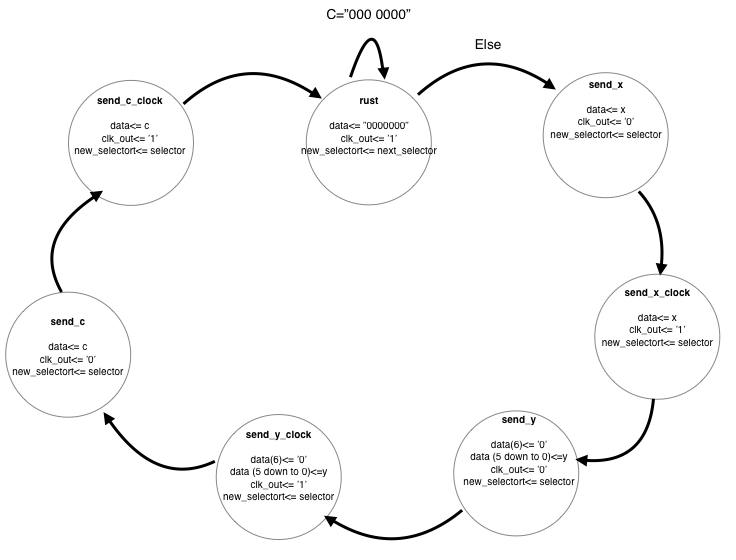
\includegraphics[width = 15cm]{Figuren/LCD/fsm_sender.png}
	\caption{FSM van component zender}
	\label{fig:fsm_zender}
\end{figure}

\subsubsection{VHDL code}
De vhdl code van de zender is opgedeeld in twee stukken, namelijk een send control en een send bus. Deze twee zijn vervolgens met een structural behaviour bij elkaar gevoegd. De code van de send control is te vinden in \ref{code:ent_send_control} en \ref{code:beh_send_control}. De code voor de send bus is te vinden in \ref{code:ent_send_bus} en \ref{code:beh_send_bus}. De top structure is te vinden in \ref{code:ent_send_top} en \ref{code:struc_send_top}.

\subsubsection{Simulaties}
De simulatie van de gehele zender is te vinden in \ref{fig:sim_sender}. Hierin is goed te zien dat ready voor elk blok apart omhoog gaat en dat het blok voor blok behandeld wordt. Deze simulatie is gedaan met de testbench in \ref{code:tb_send_top}.

\subsubsection{Resultaten}
De simulatie is zoals te verwachten valt. Hierdoor kan geconcludeert worden dat de zender naar behoren werkt.